\section{Rubin Observatory Commissioning}
\label{sec:commissioning}

\subsection{Commissioning Milestones}
\label{ssec:commissioning-milestones}

Commissioning work is being planned around two major milestones, ``First Photon'' and ``System First Light''. 

\textbf {First Photon}: Defined as the very first photons to pass through the optical system and fall on the  focal plane to produce an image of the night sky.

\textbf {System First Light}: Defined as the first science-grade images of the night sky obtained with LSSTCam. 
Also referred to as \textbf{First Light}. 
These images will be shared with the worldwide community. 

First Photon occurs following the successful completion of system integration. 
There are no quality criteria applied to the images produced for the First Photon milestone. 
First Photon  marks the start of the the on-sky engineering phase.
System First Light  marks the end of the the on-sky engineering phase and the start of the System Optimization and Science Validation phases of commissioning.
The time from First Photon to System First Light is anticipated to be three months.
During these three months, the focus will be on fine tuning the system including optical alignment and improving the image quality, collecting calibration data, and carrying out \textit{First Look} science programs. 

For a detailed description of all the commissioning milestones and the most current dates, see \citeds{dmtn-232}.

\subsection{Commissioning Schedule}
\label{ssec:commissioning-schedule}

Following the October 2023 project schedule workshop, the Rubin Construction Project is reoptimizing the sequence of integration activities based on important updates to projected subcomponent availability.
Given recent delays in the Camera ship date and important repairs needed to the summit dome crane, it will be beneficial to reinsert on-sky data taking with ComCam into the commissioning schedule for approximately two months, around July-August 2024. 
This will enable Telescope commissioning, primarily the Active Optics System, to occur approximately four months earlier than could be done with LSSTCam. 
With this updated strategy, System First Light  is projected to occur in January 2025, with Construction completion in May 2025.

\begin{figure}[htb]
\centering
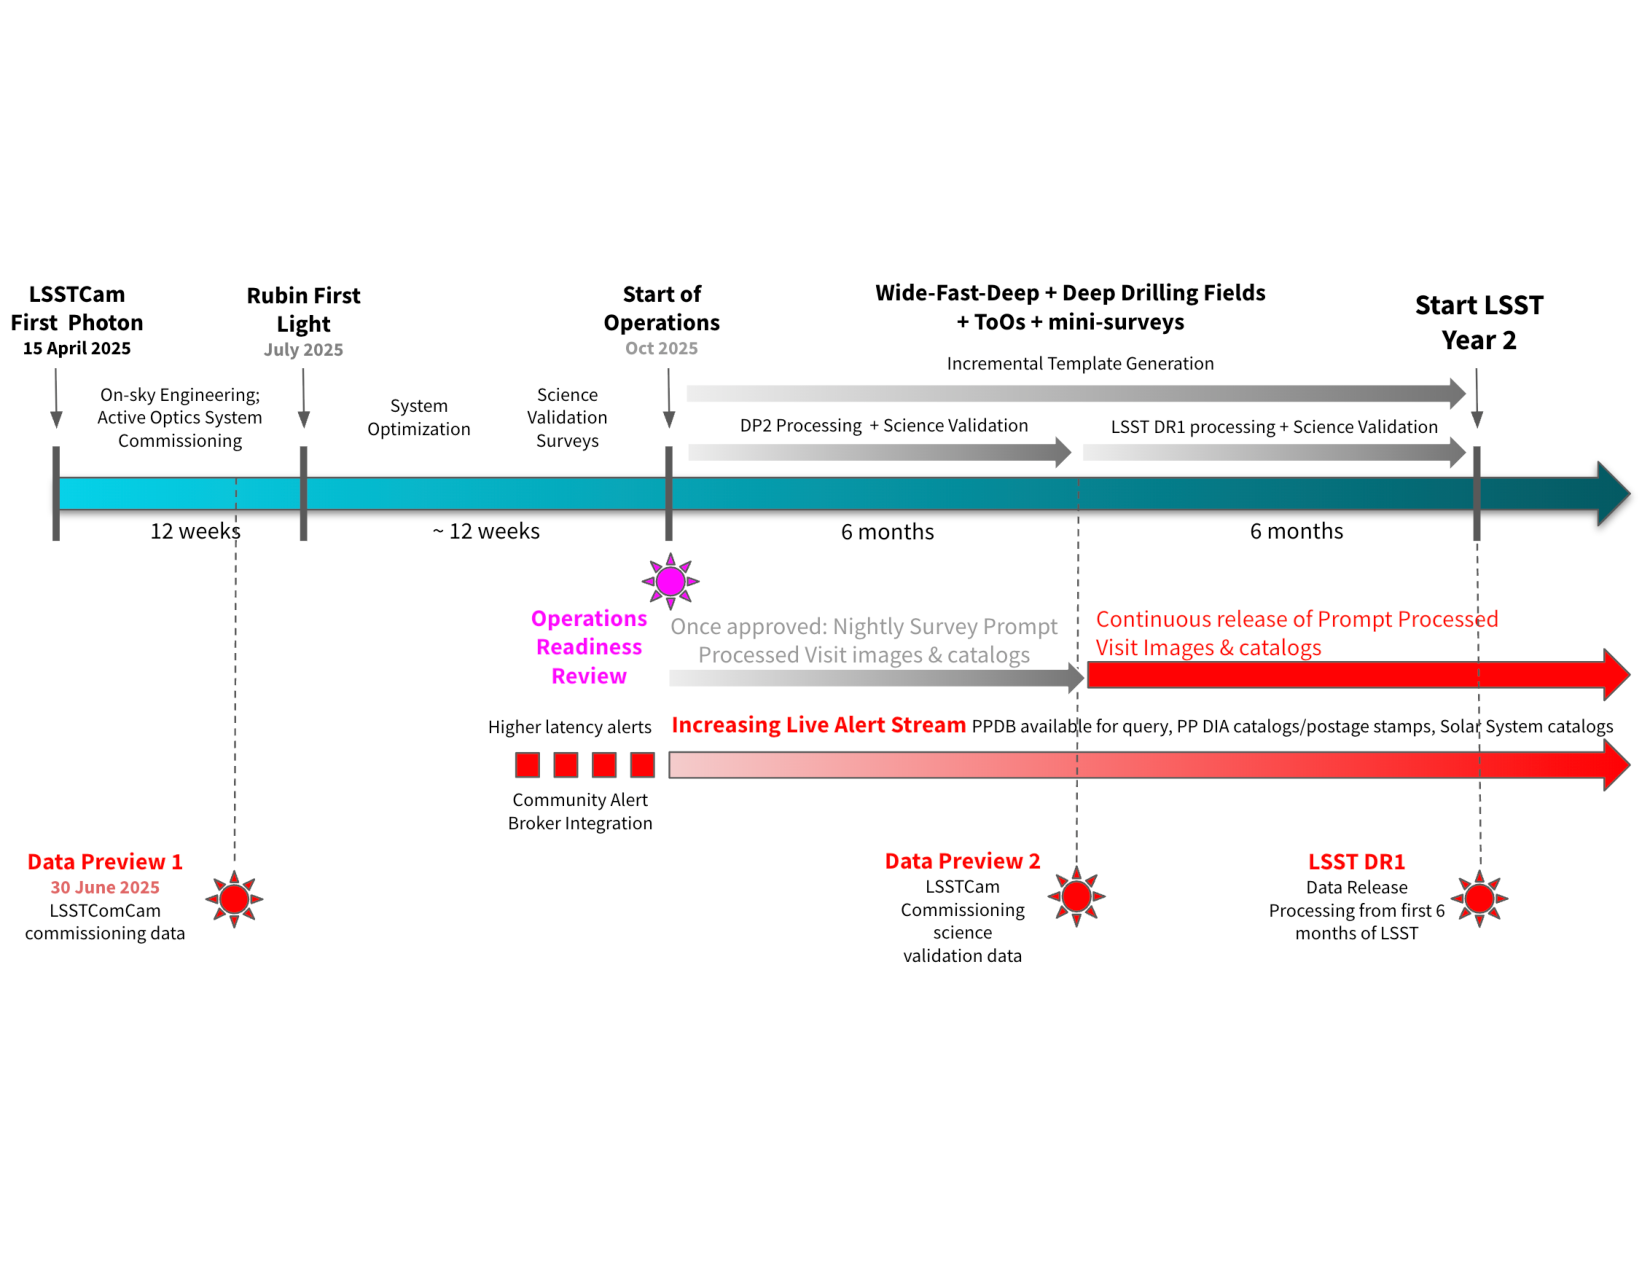
\includegraphics[width=0.98\linewidth]{figures/rubinobs_on-sky_commissioning_and_early_science.pdf}
\caption{Detailed schedule of commissioning  and early science activities relative to System First Light, as of October 2023.}
\label{fig:commissioning-es-schedule}
\vspace{0.1cm}
\end{figure}

Figure~\ref{fig:commissioning-es-schedule} shows the detailed schedule of commissioning and early science activities relative to System First Light, as of October 2023.
System First Light is currently expected in January 2025 (\S~\ref{sec:timeline}), about 3 months after on sky commissioning activities begin.
The total amount of science validation time currently planned is about 8 weeks.  
LSST data taking is expected to start 4-10 months after System First Light depending on construction schedule uncertainty and Operations readiness to start the survey following the start of full Survey Operations.
The project schedule will continue to evolve as the remaining subcomponents are delivered and the Project expects take the final decision concerning ComCam on-sky data taking in February 2024.

\subsection{Commissioning Observations}
\label{ssec:commissioning-observations}

Figure~\ref{fig:commissioning} shows the high level plan for the Rubin commissioning observations with the LSST Science Camera.
Commissioning data collection is planned to take place in phases.
Following the System First Light milestone, a set of observations designed to help optimize the system will be taken during the System Optimization phase before the Science Validation Surveys are carried out. 
The SV Surveys are designed to support scientific analyses that validate the system's performance, and allow Rubin to demonstrate operations readiness \citeds{SITCOMTN-005}.

\begin{figure}[htb]
\centering
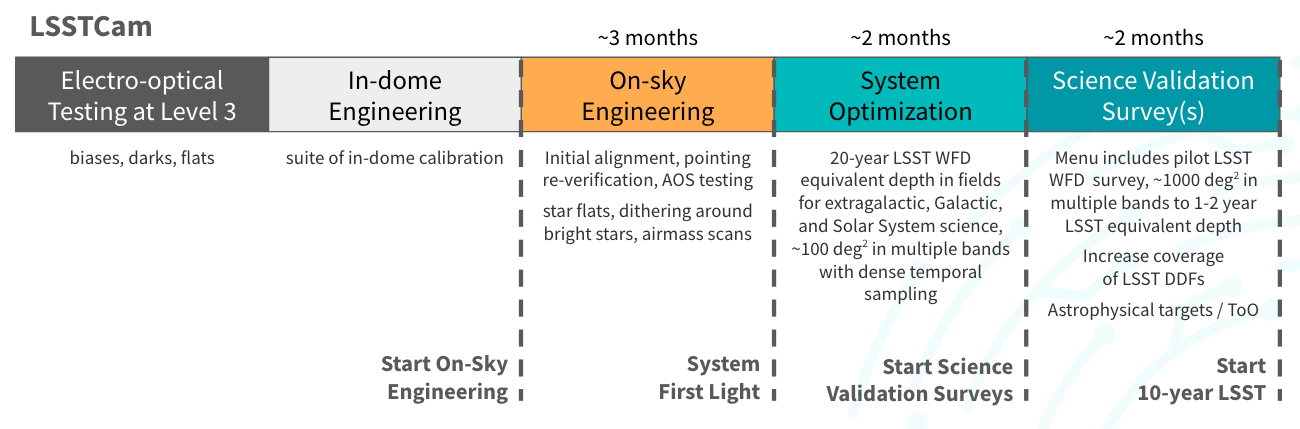
\includegraphics[width=0.95\linewidth]{figures/commissioning-plan}
\caption{Outline plan for the collection of commissioning data, as of October 2022.}
\label{fig:commissioning}
\end{figure}

Figure~\ref{fig:commissioning} also indicates a number of planned key components of the System Optimization and SV phases.
These include a LSST wide-fast-deep (WFD) 1-2 year equivalent depth ``pilot'' survey.
Field selection will be carried out by the Commissioning Team, taking into account a wide variety of constraints as well as a ``menu'' of science opportunities to which the LSST Science Community has contributed.
Details of the plans for commissioning observations will be made available as those plans converge, in this technote and other documents as cited.